\section{Milestone I}\label{sec:milestone_1}
Some introduction about what it is all about.

Cite: \citet{baumannLectureNotesCosmology2017}, \citet{dodelsonModernCosmology2003} and \citep{callinHowCalculateCMB2006, wintherCosmologyIILecture2024, huCompleteTreatmentCMB1998}

\subsection{Theory}
This study is based on the common Lambda-CDM model \citep[chap. 1][sec. 1.6]{dodelsonModernCosmology2021}, with a Friedmann-Robertson-Walker metric for spacetime.

Fiducial cosmology and initial parameter values taken from the Planck 2018 results \citep{collaborationPlanck2018Results2020}.

\subsubsection{Friedmann equation}
Rather than dealing with the full Einstein equations directly, it is possible to derive the Friedmann equation in order to describe the expansion of the universe, this is eq. \ref{eq:Friedmann} \citep{wintherCosmologyIILecture2024}.

\begin{equation}\label{eq:Friedmann}
\boxed{H = H_0 \sqrt{ \Omega_{M 0} a^{-3} + \Omega_{R 0} a^{-4} + \Omega_{k 0} a^{-2} + \Omega_{\Lambda 0}}}\,,
\end{equation}

where the $\Omega_{X}$ are density parameters describing relative density of their respective form of energy contributing to the expansion of the universe. Density parameters are dimensionless. Subscript $_0$ indicates a value for the universe of today, since we as observers are by definition at $x=a=z=0$.

$\Omega_{M} = (\Omega_{b}+\Omega_{\rm CDM})$ is a composite density parameter describing non-relativistic matter (baryons and cold dark matter), and $\Omega_{R} = (\Omega_{\gamma} + \Omega_{\nu})$ is a composite density term for radiation (photons and neutrinos).
$\Omega_{\Lambda}$ is the density parameter for dark energy.
$\Omega_{k}$ is a curvature term, and not properly an energy density. However, it contributes to the Friedmann equation as if it were a normal matter fluid with equation of state $\omega = -1/3$. This term prescribes negative curvature when $<0$, positive curvature when $>0$, and a spatially flat universe when $=0$. Our universe is observationally confirmed to be very close to flat \citep{bennettNineYearWilkinsonMicrowave2013}, so this term should be close to $0$. 

The unit of $H$ is slightly ambiguous, as in SI units both (km$/$s)$/$Mpc and the simplified $1/$s are used. The first way of writing the unit is more intuitive, as it relates to the change in velocity of distant galaxies based on their distance from the observer (us), aka Hubble's law. $1/s$ is technically correct but interpreting the Hubble parameter as a frequency is not helpful. For this project, we will in equations skip this problem by writing $H$ in "units of $H$", using the value of the Hubble parameter today ($H_0$) as a constant which gives the right units to any $H$ that pops up.

For numerical work, we calculate the constant $H_0$ by adding the right units to a dimensionless constant $h$ (eq. \ref{eq:little_h}), which is commonly used and reported in the literature \citep{crotonDamnYouLittle2013}. $h$ is one of the input observables for our numerical simulation, so we use the $0.67$ value reported by Planck 2018 \citep{collaborationPlanck2018Results2020}.

\begin{equation}\label{eq:little_h}
H_0 = 100 * h \; \text{km} \, \text{s}^{-1} \, \text{Mpc}^{-1}
\end{equation}

Equation for critical density of the universe today \ref{eq:critical_density}

\begin{equation}\label{eq:critical_density}
\rho_{c0} \equiv \frac{3H_0^2}{8\pi G} \quad \text{(kg}/\text{m}^3\text{)}
\end{equation}

\subsubsection{More stuff}

Paper with supernova fitting data \citet{betouleImprovedCosmologicalConstraints2014}

\subsection{Implementation details}
Something about the numerical work.

\subsection{Results}
Show and discuss the results.

See figs. \ref{fig:milestone_1_cosmic_vs_conformal_time}, \ref{fig:milestone_1_luminosity_distance}, \ref{fig:milestone_1_etaHp_over_c_of_x}, \ref{fig:milestone_1_Omega_i_of_x}, \ref{fig:milestone_1_supernovafitting_confidence_regions}.

\begin{figure}
\centering
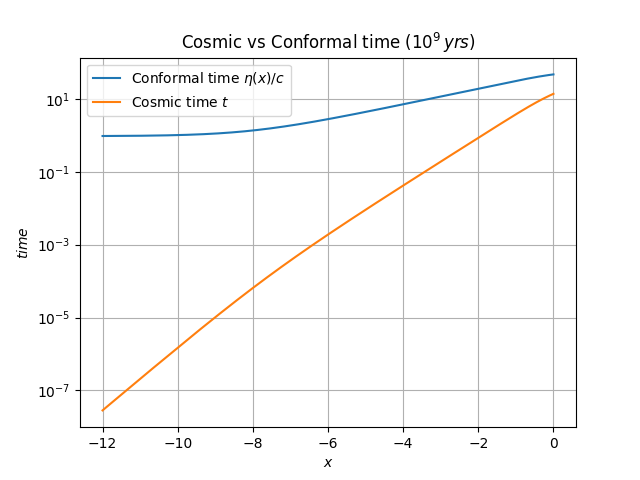
\includegraphics[width=0.4\textwidth]{../Milestone 1/Plots/cosmic_vs_conformal_time.png}
\caption{Caption}
\label{fig:milestone_1_cosmic_vs_conformal_time}
\end{figure}

\begin{figure}
\centering
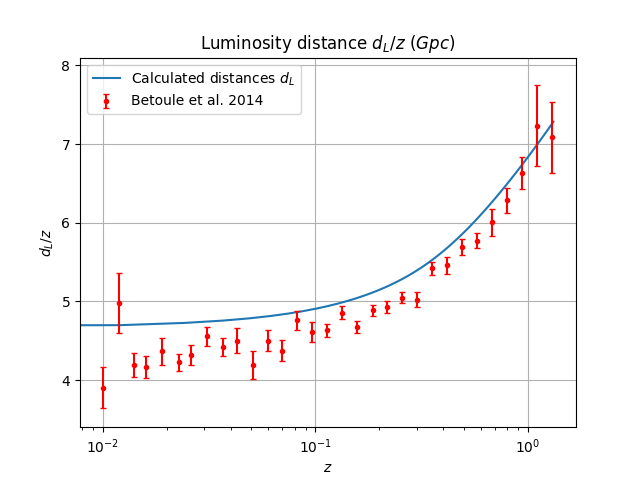
\includegraphics[width=0.4\textwidth]{../Milestone 1/Plots/luminosity_distance.png}
\caption{Caption}
\label{fig:milestone_1_luminosity_distance}
\end{figure}

\begin{figure}
\centering
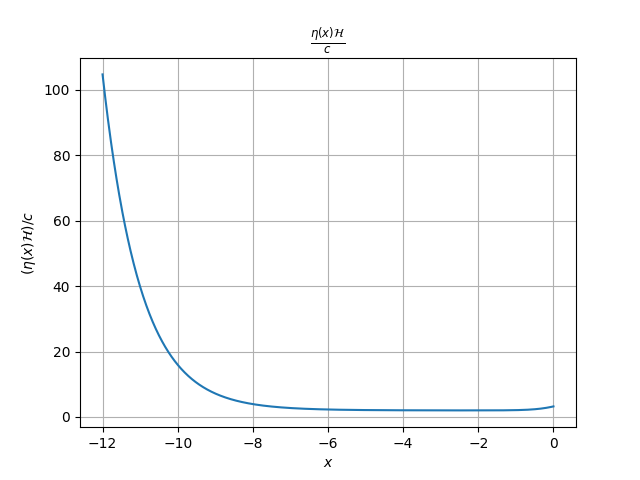
\includegraphics[width=0.4\textwidth]{../Milestone 1/Plots/etaHp_over_c_of_x.png}
\caption{Caption}
\label{fig:milestone_1_etaHp_over_c_of_x}
\end{figure}

\begin{figure}
\centering
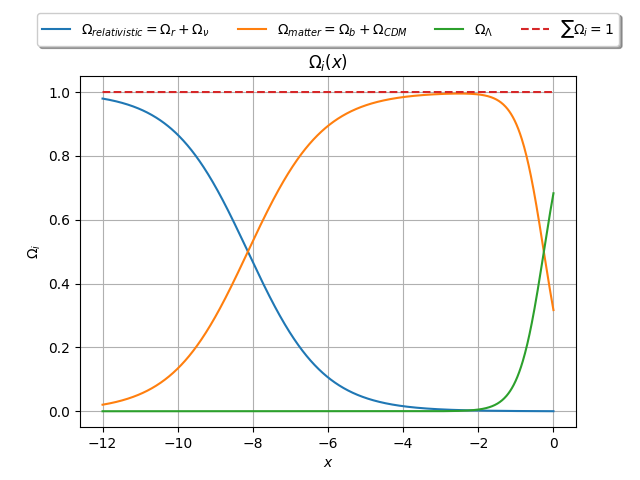
\includegraphics[width=0.4\textwidth]{../Milestone 1/Plots/Omega_i_of_x.png}
\caption{Caption}
\label{fig:milestone_1_Omega_i_of_x}
\end{figure}

\begin{figure}
\centering
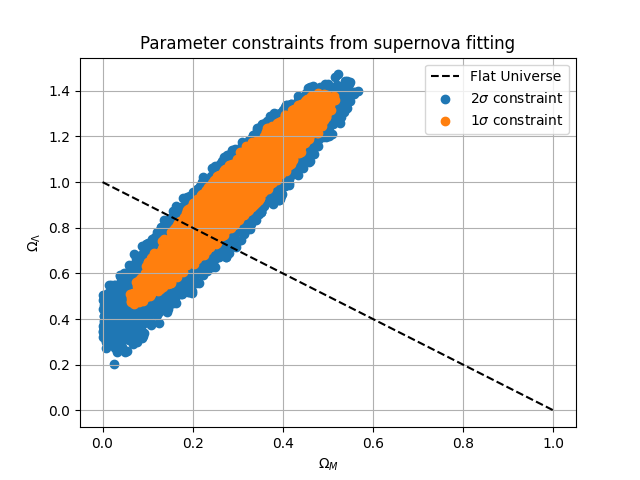
\includegraphics[width=0.4\textwidth]{../Milestone 1/Plots/supernovafitting_confidence_regions.png}
\caption{Caption}
\label{fig:milestone_1_supernovafitting_confidence_regions}
\end{figure}
